\chapter{Introduction}

\section{Figures}

Place your image in chapters/images folder. Refer \ref{fig:waterfall}
\begin{figure}
	\centering
	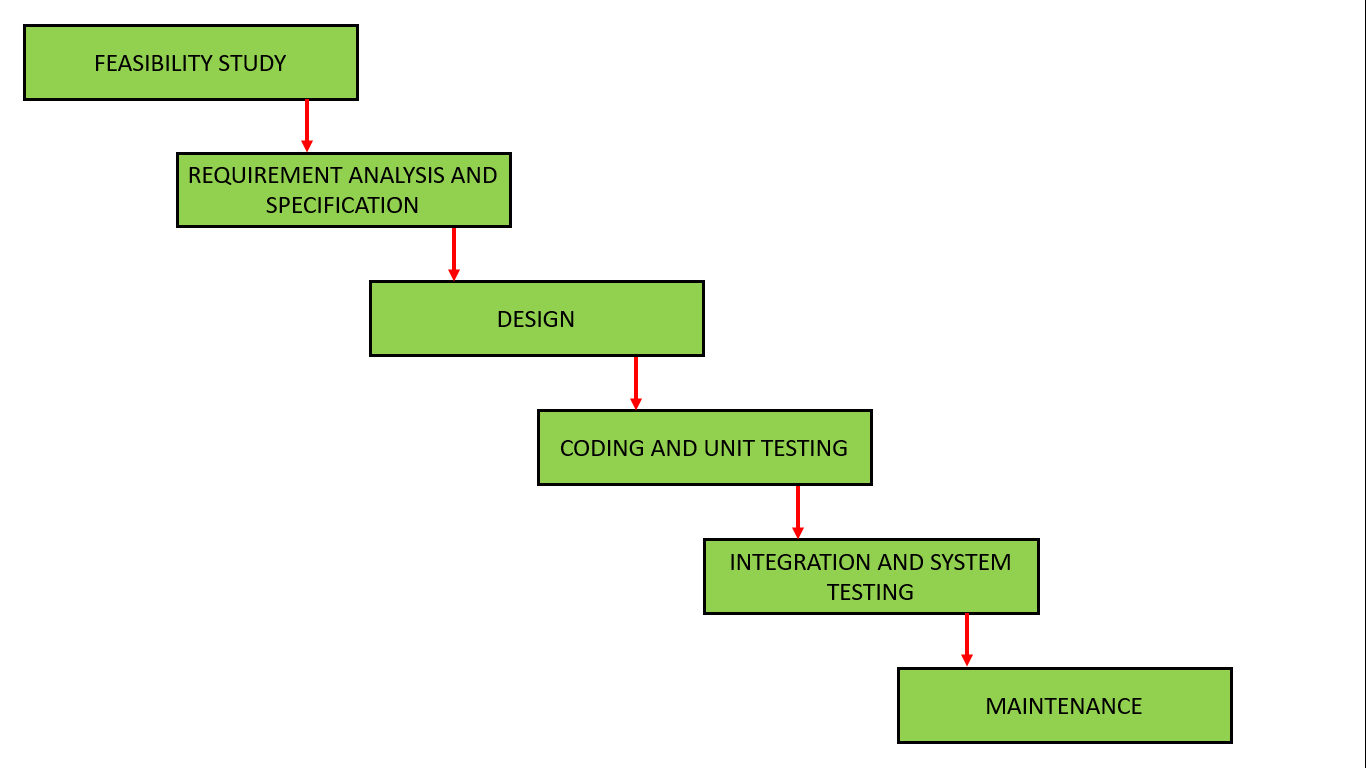
\includegraphics[scale=0.15]{chp/images/waterfall.png}
	\caption{Various stages involved in the waterfall model}
	\label{fig:waterfall}
\end{figure}

\section{Code snippets}
Place your code snippets in codes folder. Refer \ref{fig:sample_code} 
\begin{figure}

	\begin{lstlisting}
		#include <iostream>
		
		int main() {
			std::cout << "Hello, World!" << std::endl;
			return 0;
		}
	\end{lstlisting}

	\caption{Sample function.}
	\label{fig:sample_code}
	\begin{figure}


\section{Tables}
\begin{table}
	\centering
	\begin{tabular}{l|l}
		A & B \\
		\hline 
		1 & 2 
	\end{tabular}
	\caption{Sample table}
	\label{tab:highlights}
\end{table}

\section{Abbreviations}
Abbreviation

\section{Footnotes}
You can add footnotes \footnote{Sample footnote}
You can also add another \footnote{Second Footnote}

\section{References}
Add BibTeX format bibliography entries in bib.bib and cite anywhere like this; \cite{sample_cite}
According to \cite{knuth1984texbook}, LaTeX is a powerful typesetting system.
In the above example, the BibTeX entry is for a journal article titled "A Mathematical Theory of Communication" by Claude E. Shannon, published in the Bell System Technical Journal in 1948. The article was published in volume 27, issue 3, and it spans pages 379-423 and 623-656. The reference includes a DOI number, which can be used to access\cite{sample_cite} the article online.  third reference \cite{Shannon1948}. The another level of text is here. The another \footnote{sample footnote text} reference is to be kept here
According to \cite{Shannon19482}, information theory is a mathematical framework for understanding communication systems.

The another level \footnote{foot3} of text is here.



